\newcommand{\dpop}{\Delta p/p}

Изначальной целью экспериментов по изучению времени когерентности спина (Spin Coherence Time) на COSY было подтверждение
возможности секступольных полей противодействовать дисперсии спин-тюнов, ассоциированной с 
эмиттансом и дисперсией импульсов ($\dpop$) частиц пучка.~\cite{COSY:SCT:IPAC15} На настоящий момент, оптимизация SCT является первой фазой любого предварительного эксперимента по поиску ЭДМ на COSY.

Секступольное подавление декогеренции используется совместно с электронным охлаждением пучка, для
уменьшения его фазового объёма, и банчингом, для подавления линейного вклада дисперсии импульсов частиц 
в декогеренцию. Секступоли, располагающиеся в арках, призваны подавлять эффект декогеренции второго порядка.

Для контроля декогеренции используются три семейства секступолей, которые маркированны соответственно: MXG, расположенный в максимуме дисперсионной функции, и контролирующий эффект декогеренции связанный с $\dpop$; MXS, расположенный в максимуме горизонтальной бета-функции $\beta_x$, и контролирующий дисперсию, связанную с горизонтальными бетатронными колебаниями; MXL, в максимуме $\beta_y$, контролирующий дисперсию, возникающую из-за вертикальных бетатронных колебаний.

\begin{figure}[h]\centering
	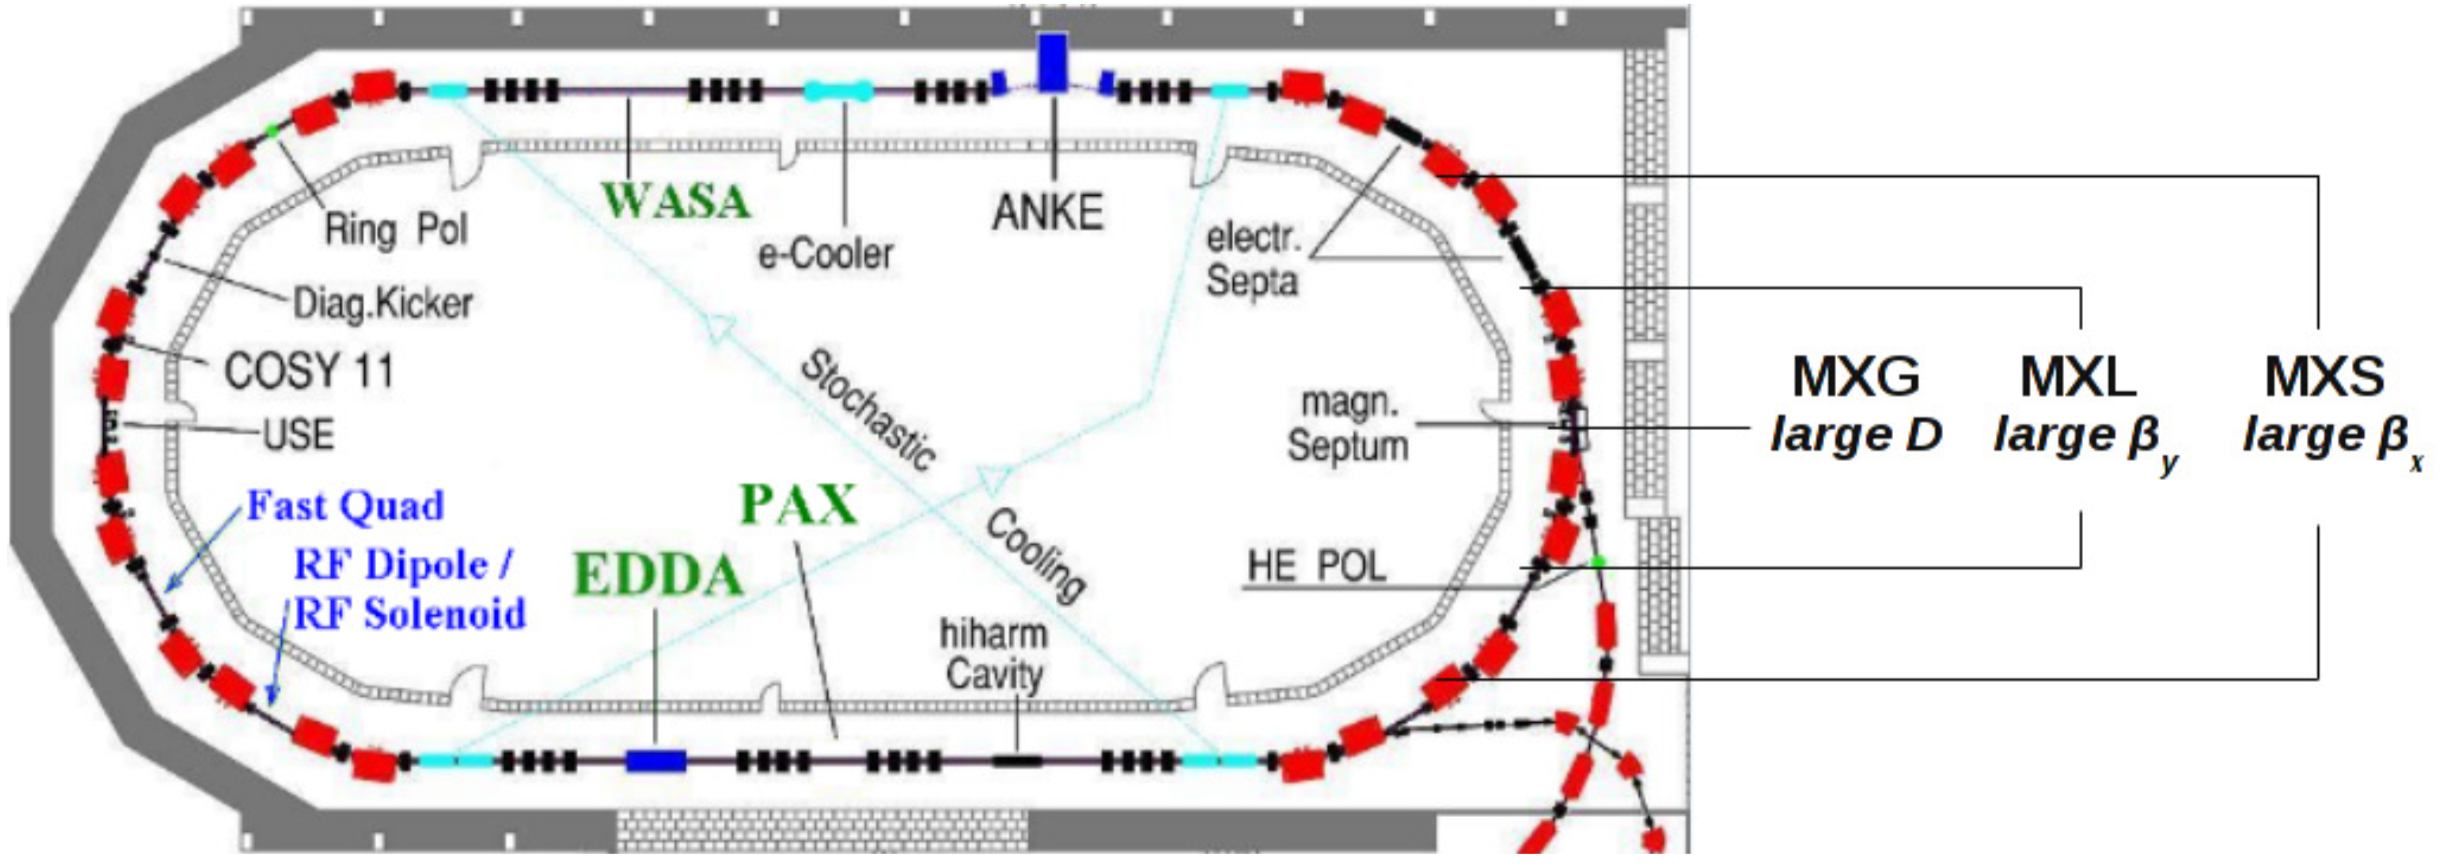
\includegraphics[width=\linewidth]{images/chapter4/COSY-sextupoles}
	\caption{Кольцо COSY с отмеченными положениями секступолей для контроля времени когерентности спина. (Рисунок взят из~\cite{Guidoboni:STORI14}.)}
\end{figure}

\subsection{Процедура оптимизации}
В этом разделе описана процедура оптимизации SCT, на примере эксперимента 2014 года.~\cite{Guidoboni:STORI14} Первый оптимизационный эксперимент проводился в 2012 году, но тогда варьировалась только напряжённость поля секступоля MXS. В 2014 году впервые проведён полноценный (варьировались градиенты всех трёх секступолей) эксперимент по оптимизации SCT. 

Чтобы отделить эффекты декогеренции, связанные с конечностью эмиттанса пучка, и с вторым порядком дисперсии импульсов частиц $(\dpop)^2$, подготовка пучка к эксперименту проводится по-разному.

Для получения пучка с большим разбросом $(\dpop)^2$, поляризованный дейтронный пучок с импульсом $p=0.97$ ГэВ/с сначала охлаждается в течении 60 секунд для минимизации его эмиттанса. После отключения охлаждения пучок банчируется (гармоническое число $h=1$). Банчирование необходимо для подавления линейных эффектов декогеренции.

В случае изучения декогеренции, связанной с горизонтальным эмиттансом пучка,~\footnote{Декогеренция, связанная с вертикальным эмиттансом не может быть изучена ввиду ограничений по аксептансу.} охлаждение и банчирование проводятся одновременно в течении первых 60 секунд, после чего охлаждение отключается, и на пять секунд включается горизонтальное нагревание. Пучок нагревается подачей белого шума на обкладки конденсатора горизонтального кикера.

В обоих случаях, пучок инжектируется с вертикально-ориентированным вектором поляризации. Поворот поляризации в горизонтальную плоскость производится ВЧ соленоидом, после подготовки пучка, на 80-й секунде.

Мониторинг поляризации пучка производится непрерывно, путём приложения белого шума на вертикальный кикер, для экстракции пучка на 17-мм углеродную мишень. Далее, эластично-рассеянные дейтроны детектируются на поляриметре EDDA. Эластичное рассеяние дейтронов на углеродной мишени чувствительно к направлению спина, и имеет большое сечение взаимодействия. 

Сцинтилляторы поляриметра поделены на четыре группы: верхние, нижние, левые, правые; асимметрия частот событий на левом и правом детекторах пропорциональна вертикальной поляризации, а на верхнем и нижнем --- горизонтальной поляризации. Прецессия поляризации пучка в горизонтальной плоскости происходит с частотой, значительно превышающей частоту выборки поляриметра, поэтому в 2012 году была разработана специальная система сбора данных~\cite{COSY:SCT:DAQ}.

По результатам эксперимента 2014 года~\cite{Guidoboni:STORI14} была доказана возможность получать на COSY SCT свыше 1,000 секунд. 

\paragraph{Изменение SCT при переходе от halo- к core-части пучка}
Ниже представлены результаты  этой процедуры, полученные в период измерений апрель-май 2019 года.